\chapter{Erarbeitung des Konzepts}\label{ch:conception}
Bevor mit der eigentlichen Implementierung begonnen werden kann wird ein grober Plan erstellt.
In diesem Plan beziehungsweise Konzept wird die Art und Weise, wie die Anwendung funktionieren soll, definiert und gegebenenfalls werden UI-Prototypen erstellt.\pbreak%
%
Dieses Kapitel wird im Allgemeinen in die drei Hauptbereiche der Anwendung unterteilt, in denen die Ideen der Funktionsweise erklärt werden.
Dazu gehört das Erstellen und Verwalten von Projekten, das Bearbeiten und Zeichnen der eigentlichen Kartendaten und das Exportieren eines fertigen Projektes in das \acl{imdf}.
Diesen drei Abschnitten ist das Design-Konzept vorangestellt, in dem die Grundlagen für das Design der Benutzeroberfläche beschrieben werden.\pbreak%
%
Nach einigen Überlegungen und verschiedenen Arbeitstiteln wurde sich für den Anwendungsnamen \textbf{Indoor Architect} entschieden.
Somit wird in den folgenden Abschnitten mit Indoor Architect die Anwendung gemeint.

\section{Design-Konzept}
In diesem Abschnitt werden die allgemeinen Fragen bezüglich des Design von Indoor Architect beschrieben.
Dabei wird genauer auf die Navigation durch die Anwendung eingegangen.
Im Anschluss wird vor allem die Trennung des Kartenbereichs von dem Rest der Anwendung genauer erklärt und die gewählten Farben dargestellt.\pbreak%
%
Anders als bei den analysierten aktuellen Lösungen aus \autoref{ch:analysis} soll Indoor Architect so minimalistisch wie möglich werden.
Trotzdem sollen alle wichtige Funktionen zur Erstellung von Indoor Maps enthalten bleiben.
Der Benutzer darf sich nicht in einem Projekt gefangen fühlen und sollte zu jeder Zeit ohne großen Aufwand zwischen verschiedenen Projekt wechseln können.

\subsection{Navigation}
Die Navigation durch die Anwendung wird mittels Push- und Pop-Navigation erreicht.
Dabei gibt es eine Hauptansicht, von der man in verschiedene Unteransichten navigieren kann und ebenso wieder zurück navigieren kann.
Der Vorteil gegenüber anderen Arten der Navigtion ist, dass es nur einen Pfad zu jeder Ansicht gibt und man daher besser im Blick behalten kann wo man sich befindet.
Dadurch kann in den folgenden Abschnitten ein Navigationsbaum erstellt werden, welcher die Navigations in den Bereichen beschreibt.\pbreak%
%
Um dem vorher beschreibenen Punkt gerecht zu werden, dass man schnell und einfach zwischen verschiedenen Projekten wechseln können sollte wird eine Seitenleiste vorhanden sein.
In dieser Seitenleiste werden die Projekte und gegebenenfalls weitere Punkte aufgelistet über die man einen anderen Kontext öffnen kann.
\begin{figure}[h!]
	\centering
	\vspace{15pt}
	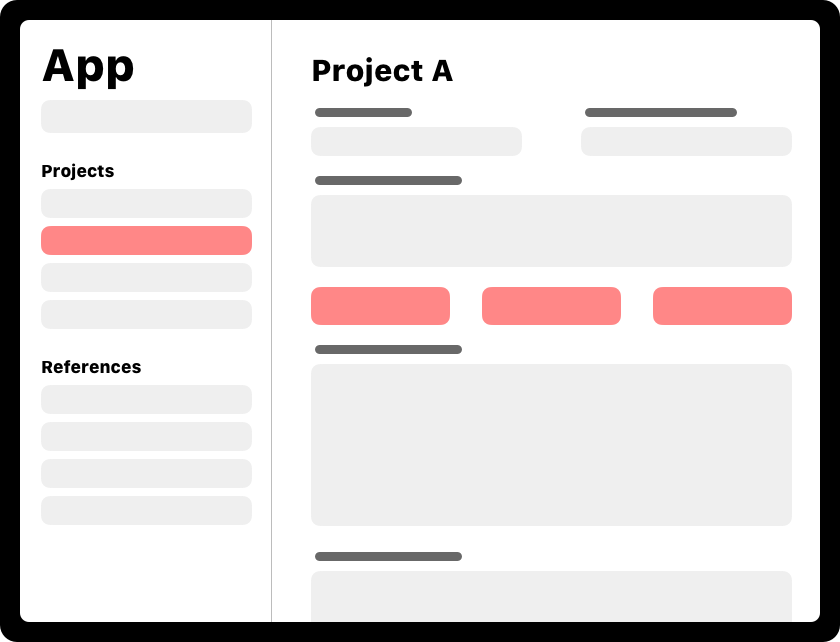
\includegraphics[scale=0.4]{images/design-app}
	\caption{Mockup der Hauptansicht eines Projektes}
	\label{fig:design-app}
\end{figure}
In der Abbildung \ref{fig:design-app} erkennt man, dass in der Seitenleiste auf der linken Seite das zweite Projekt (Project A) ausgewählt ist und auf der rechten Seite die Projektübersicht dargestellt wird.
Auf der rechten Seite kann der Benutzer nun das Projekt verwalten und Unteransichten öffnen, die in dem rechten Bereich angezeigt werden.
Die Seitenleiste bleibt weiterhin sichtbar, sodass globale Funktionen der Anwendung – wie die Einstellungen, das Durchsuchen der Anwendung oder das Erstellen eines neuen Projektes – zu jeder Zeit zugänglich sind.
Selbst wenn der Benutzer sich in tieferen Ebenen der Projekteinstellungen wiederfindet ist ihm stets klar in welchem Projekt er gerade navigiert.

\subsection{Trennung des Kartenbereichs}
Eine Ausnahme dabei ist der Kartenbereich.
Wenn ein Benutzer die Kartendaten eines Projektes bearbeiten möchte, muss der Karteneditor geöffnet werden.
Da für das Bearbeiten der Kartendaten eine möglichst große Fläche von Vorteil ist, wurde sich dazu entschieden dem Karteneditor den kompletten Bildschirm bereitzustellen.
Dem Benutzer wird dann nur der Kartenkontext angezeigt, sodass er sich auf diesen Bereich konzentrieren kann.
In der Abbildung \ref{fig:design-map} findet man in der oberen linken Ecke einen Schließen-Button, welcher den Karteneditor wieder schließt und den Benutzer zurück zur Projektübersicht bringt.
\begin{figure}[h!]
	\centering
	\vspace{15pt}
	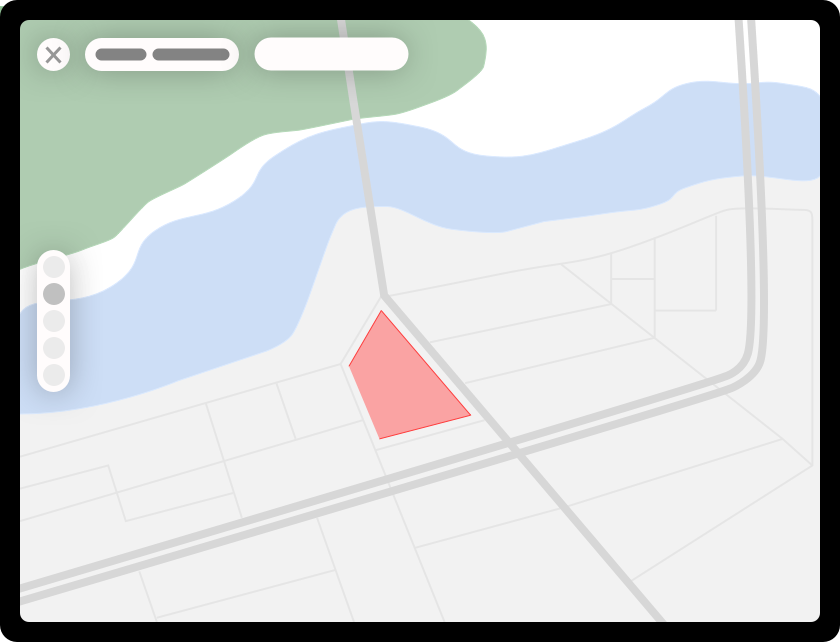
\includegraphics[scale=0.4]{images/design-map}
	\caption{Mockup der Kartenansicht eines Projektes}
	\label{fig:design-map}
\end{figure}

\subsection{Barrierefreiheit}
Für die Entwicklung von Indoor Architect ist es wichtig, dass auf die Barrierefreiheit geachtet wird.
Dies bedeutet unter anderem auf entsprechend hohe Kontrastwerte zwischen den verwendeten Farben zu achten und die Schriftgrößen richtig zu wählen.
Um die Ziele der Barrierefreiheit zu erreichen, kann man die bereits vorhandenen Schnittstellen des genutzten \Gls{sdk} verwenden.\pbreak%
%
Anstatt für einen Text eine Schriftart und Schriftgröße zu wählen, wählt man eine semantische Kategorie für den Textbereich (zum Beispiel \emph{Überschrift} oder \emph{Fließtext}).
Der Benutzer, welcher Funktionen der Barrierefreiheit nutzt und in seinen Geräteeinstellungen zum Beispiel eine größere Schrift eingestellt hat, wird auch in der Anwendung eine für ihn ansprechende Schrift wiederfinden anstatt die festgelegte Schriftgröße.
Ebenso kann das System die Schriftstärke je nach Präferenz des Benutzers wählen, wenn man dynamische Schriften erlaubt und die Stärke nicht manuell setzt.\pbreak%
%
Gleiches gilt für die Verwendung von Farben.
Wenn in Indoor Architect Farben verwendet werden, dann müssen diese aus vier unterschiedlichen Farben bestehen.
Zum einen lässt sich zwischen einem hellen und einem dunklen Modus wechseln, zum anderen gibt es für Benutzer mit Sehschwächen in den Geräteeinstellungen die Möglichkeit eine \emph{High Contrast}-Einstellung zu wählen.
Damit Indoor Architect diese Funktion der Barrierefreiheit unterstützen kann, muss für jede Farbe auch immer eine \emph{High Contrast}-Variante bereitsgestellt werden.
Daraus ergeben sich folgende vier Kombinationen pro Farbe:
\begin{itemize}
	\setlength\itemsep{0pt}
	\item[] \colorbox{redL}{\color{white}\texttt{\#ff3b30}\hspace{20pt}} \hspace{10pt}Normaler Kontrast
	\item[] \colorbox{redDL}{\color{white}\texttt{\#ff453a}\hspace{20pt}} \hspace{10pt}Dunkelmodus, Normaler Kontrast
	\item[] \colorbox{redH}{\color{white}\texttt{\#d70015}\hspace{20pt}} \hspace{10pt}Hoher Kontrast
	\item[] \colorbox{redDH}{\color{white}\texttt{\#ff6961}\hspace{20pt}} \hspace{10pt}Dunkelmodus, Hoher Kontrast
\end{itemize}
Die dargestellten Farbkombinationen sind die der vom System bereitgestellten Farbe Rot (\texttt{systemRed}).
Je nach Geräteeinstellung des Benutzers wird die entsprechende Farbe für den normalen oder den Hochkontrastmodus gewählt und angezeigt.\pbreak%
%
Neben der automatischen Anpassung der dargestellten Schrift und Farben gibt es noch weitere Möglichkeiten wie die Barrierefreiheit für Benutzer verbessert werden kann.
Ein weiterer Schritt könnte das Vermeiden von Transparenzen und Animationen sein.
In den \emph{Human Interface Guidelines} für iOS-Anwendungen, welche Empfehlungen und Ressourcen für das UI-Design auf Apple-Plattformen bereitstellen, weist Apple darauf hin, dass Transparenzen und Animationen für einige Personen ablenkend oder sogar unangenehm sein können \parencite{APP2020a}.
Da keine starken Transparenzen in Indoor Architect eingebaut werden und die Animationen, die verwendet weden, bereits auf Barrierefreiheit achten, müssen dafür keine Schritte vorgenommen werden.
Für Benutzer die an Blindheit leiden gibt es zudem noch die \emph{VoiceOver}-Funktion, welche berührten Fließtext sowie unter anderem den Titel von Buttons vorließt.
Um die Aktion hinter dem Button auszuführen muss ein zweites mal auf den Button geklickt werden.
Auch in diesem Fall kann diese Barrierefreiheitfunktion außer acht gelassen werden, da die Betroffenen nicht Zielgruppe der Anwendung sind.
Selbst mit den entsprechenden Funktionen der Barrierefreiheit ist das Zeichnen auf den Kartendaten mit einer Blindheit in dieser Anwendung schwer zu verwirklichen.

\section{Erstellen von Projekten}
Navigationsbaum\\
Verweise auf Anhänge\\
Eingabe von Titel, Client und Description\\
Eingehen auf das Format, wie das Projekt gespeichert werden soll (JSON, Struktur)
\section{Bearbeiten der Kartendaten}
Navigationsbaum (Eingehen auf die andere Art der Navigation)\\
Beschreiben der Tools für die Bearbeitung\\
Anklicken von Items öffnet die Edit Form
\section{Ausführen eines Audits}
Navigationsbaum\\
Erklärung der Validation Rules\\
Anzeige mit Lösungsvorschlägen\\
Automatisches Resolven von Issues
\section{Exportieren der Projekte}
Export als IMDF Format\\
Export als Indoor Architect Archiv
